\documentclass[12pt]{article}
\usepackage[T1]{fontenc}
%\usepackage[latin9]{inputenc}
\usepackage[utf8]{inputenc}
\usepackage[english]{babel}
\usepackage{amsmath}
\usepackage{amsfonts}
\usepackage{amssymb}
\usepackage{setspace}
\usepackage{rotating}
\usepackage{graphics}
\usepackage[round]{natbib}
%\usepackage{graphicx}
%\usepackage{float} 				%allows you to float images
\usepackage{latexsym}
\usepackage{bbding}
%\usepackage {moresize}
\usepackage{listings}
\usepackage{bbding}
\usepackage{blindtext}
\usepackage{hhline}
\usepackage{tikz}
\usetikzlibrary{trees}
%\usetikzlibrary{shapes,backgrounds}
%\usepackage{pgfplots}
%\usetikzlibrary{arrows}
\usepackage{enumitem}
\doublespacing
%\usepackage{geometry}
\usepackage{amsthm}
\usepackage{color}
%\usepackage{array,multirow}
%\usepackage{subcaption}
%\usepackage{pst-plot}
%	\psset{xunit=15mm}
%\geometry{verbose,tmargin=1in,bmargin=1in,lmargin=.5in,rmargin=.5in}
\setlength{\parskip}{\bigskipamount}
\setlength{\parindent}{0pt}
\usepackage{multicol}

\newenvironment{problem}[3][Problem]{\begin{trivlist}
\item[\hskip \labelsep {\bfseries #1}\hskip \labelsep {\bfseries #2.}]}{\end{trivlist}}

\newcommand{\barr}{\bar{r}}
\newcommand{\infsum}{\sum_{n=1}^{\infty }}

\title{Problem Set 7 \thanks{Problems: 2,5,6,8,9}}
\author{Ian McGroarty \\
	Course Number: 625.641}
\date{July 16, 2019}

\begin{document}

\maketitle
\section{Theorems}
\underline{Theorem 3.9.2 (Larsen Marx (2018) page 184)}: Let X and Y be any two random variables, and let a and b be constants. Then: $$ E(aX+bY)=aE(X)+bE(Y)$$ 

\underline{Theorem 3.9.5 (Larsen, Marx (2018) page 188)} Suppose X and Y are random variables with finite variances, and a and b are constants. Then $$ Var(aX+bY) = a^2Var(X) + b^2Var(Y) + 2abCov(X,Y)$$

\underline{Proposition 1  (notes module 7)} Suppose X follows a normal distribution with mean $\mu $ and standard deviation $\sigma $. Then $$VaR_h(X) = -\sigma F_N^{-1}(h) - \mu $$

\underline{Definition: Conditional Value at Risk (notes module 7)} of a position X is the conditional expectation values of the associates loss of X given that the losses are at least equal to its value at risk: $$ CVaR_h(X) CVaR_h(X) = E[-X|X \leq - VaR_h(X)]$$

\underline{Definition: Expected Value (Larsen, Marx (2018) page 138)} Let Y be a continuous random variable with pdf $f_Y(y)$, $E(Y) = \mu = \mu_Y = \int_{-\infty }^{\infty } y \cdot f_Y(y)dy$
\newpage
%%%%%%%%%%%%%%%%%%%%%%%%%%%%%%%%%%%%%%%%%%%%%%%%%%%%%%%%
%%%%%%%%%%%%%%%%%%%%%%%%%%%%%%%%%%%%%%%%%%%%%%%%%%%%%%%%
%%%%%%%%%%%%%%%%%%%%%%%%%%%%%%%%%%%%%%%%%%%%%%%%%%%%%%%%
\begin{problem}{2}.  Suppose X is a normal with zero mean and standard deviation of \$10 million: \\
\textbf{(a)} Find the value at risk for X for the risk tolerances $h= 0.01, 0.02,0.05,0.10,0.50,0.60,$ and 0.95. \textbf{Solution:} See figure 1. \\
\textbf{(b)} Is there a relation between VaR for values of $h\leq 0.50 $ and values for $h \geq 0.50 $ \\
\textbf{Solution}
Well it seems that 0.5 is the 0 point. Values $h \leq 0.5$ are associated with a positive value at risk and values $g \geq 0.5$ are associated with negative values at risk. It also appears that they are invereses of eachother which makes sense since it is $(1-h)$. Since X is normal, there is symmetry about the mean. 
\begin{figure}[h]
\caption{Value at Risk for various Risk Tolerances}
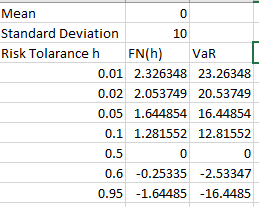
\includegraphics{mod7p2}
\centering
\end{figure}


\end{problem}
%%%%%%%%%%%%%%%%%%%%%%%%%%%%%%%%%%%%%%%%%%%%%%%%%%%%%%%%
%%%%%%%%%%%%%%%%%%%%%%%%%%%%%%%%%%%%%%%%%%%%%%%%%%%%%%%%
%%%%%%%%%%%%%%%%%%%%%%%%%%%%%%%%%%%%%%%%%%%%%%%%%%%%%%%%
\newpage
\begin{problem}{5}.  Suppose $X_1$ and $X_2$ are jointly normal positions with parameters $\mu_1,\mu_2,\sigma_1,\sigma_2,\sigma_{12}$. Show that: $ VaR_h(X_1 +X_2) \leq VaR_h(X_1) + VaR_h(X_2)$
\begin{align*} 
VaR_h(X_1 +X_2) &\leq VaR_h(X_1) + VaR_h(X_2) \\
-\sigma_{12} F_N^{-1}(h) - \mu_{12} &\leq -\sigma_{1} F_N^{-1}(h) - \mu_{1} + -\sigma_{2} F_N^{-1}(h) - \mu_{2}  && \text{Proposition 1 in notes} \\
\mu_{12} &= \mu_1 + \mu_2 && \text{By Theorem 3.9.2. Thus:} \\
-\sigma_{12} F_N^{-1}(h) &\leq -\sigma_{1} F_N^{-1}(h) + -\sigma_{2} F_N^{-1}(h) \\
-\sigma_{12} &\leq \sigma_1 + \sigma_2  \\ 
-\sigma_{12}^2 &\leq (\sigma_1 + \sigma_2)^2 && \text{Square both sides}  \\ 
Var(X) + Var(Y) + &2Cov(X,Y) \leq \sigma_1^2 + 2\sigma_1\sigma_2 + \sigma_2^2  &&\text{Theorem 3.9.5}\\
2Cov(X,Y) &\leq 2\sigma_1\sigma_2 \\
\rho \sigma_1\sigma_2 \leq \sigma_1\sigma_2 
\end{align*} 
\end{problem}
%%%%%%%%%%%%%%%%%%%%%%%%%%%%%%%%%%%%%%%%%%%%%%%%%%%%%%%%
%%%%%%%%%%%%%%%%%%%%%%%%%%%%%%%%%%%%%%%%%%%%%%%%%%%%%%%%
%%%%%%%%%%%%%%%%%%%%%%%%%%%%%%%%%%%%%%%%%%%%%%%%%%%%%%%%
\newpage
\begin{problem}{6}   Find $AVaR_h(X)$ for the X of Exercise 3. (Also see Exercise 9.) 	 \\
\textbf{Solution} We know that the density of X is $f(x) = \frac{1}{60--40} = \frac{1}{100}$ for $x \in (-40,60)$ because it is uniform. The distribution function is $F_X(x) = \frac{x+40}{100}$ for $ x \in (-40,60)$. So we have $F_X^{-1}(h) = 100h - 40.$ Therefore the Value at Risk is $$ VaR_h = -F_X^{-1}(h) = 40-100h$$

The Average value at Risk is 
\begin{align*}
 AVaR_h(X) &= \frac{1}{h} \int_0^hVaR_u(X)du \\
 &= \frac{1}{h} \int_0^h  40-100h \\
 &= 40-50h
 \end{align*}

\end{problem}


%%%%%%%%%%%%%%%%%%%%%%%%%%%%%%%%%%%%%%%%%%%%%%%%%%%%%%%%
%%%%%%%%%%%%%%%%%%%%%%%%%%%%%%%%%%%%%%%%%%%%%%%%%%%%%%%%
%%%%%%%%%%%%%%%%%%%%%%%%%%%%%%%%%%%%%%%%%%%%%%%%%%%%%%%%
\newpage
\begin{problem}{8}.  Let X be a position with a probability distribution F that is strictly increasing and smooth. Let $f(x) = F'(x)$ be the associated probability density. \\
\textbf{(a)} Verify that $CVaR_h(X) = -\frac{1}{h}\int_{-\infty }^{-VaR_h(X)}xf(x)dx $

\textbf{Solution} By Def CVaR: $CVaR_h(X) = E[-X|X \leq - VaR_h(X)] $. This is equivalent to: $E[-X] \; s.t. \; x \in (-\infty , - VaR_h(X)]$. So by Def. Expected Value $$ E[-X] = \int_{-\infty }^{- VaR_h(X)} f_X(x) \cdot x $$
Since VaR  is based on the h quantile we multiply by $1/h$?

\textbf{(b)} For any $u \in (0,1)$ let $x=F^{-1}(u)$ be the value oof X that defines the u-quantile of X. Conversely, for any specific value x of X, we have $u=F(x)$ as the quantile value associates with x Using the change of variable $u=F(x)$ in the equation (of part a) show that:
$ CVaR_h(X) = -\frac{1}{h}\int_0^h F^{-1}(u)du$
\begin{align*}
\frac{1}{h}\int_{-\infty }^{- VaR_h(X)} f_X(x) \cdot x &= \frac{1}{h}\int_{-\infty }^{- VaR_h(F^-(u))} f_X(F^-(u)) \cdot F^-(u) \\
&= \frac{1}{h}\int_{-\infty }^{- VaR_h(F^-(u))}  F^-(u) du 
\end{align*}
To determine $- VaR_h(F^-(u))$: $h = P(-X>V) = P(-F^-(u) > V) = P(F^-(u) \leq V) = P(u \leq F(V)) =  F(F^-(V)) = V \implies VaR(x) = h?$ Thus,  $ CVaR_h(X) = -\frac{1}{h}\int_0^h F^{-1}(u)du$


\textbf{(c)} Interpret the right hand side of equation (in part b) to obtain: 
$$AVaR(X) = -\frac{1}{h}\int_0^h F^{-1}(u)du$$
and hence conclude that $CVaR_h(X) = AVaR_h(X)$.
\textbf{Solution} Does anything need to be done here? 
\end{problem}

%%%%%%%%%%%%%%%%%%%%%%%%%%%%%%%%%%%%%%%%%%%%%%%%%%%%%%%%
%%%%%%%%%%%%%%%%%%%%%%%%%%%%%%%%%%%%%%%%%%%%%%%%%%%%%%%%
%%%%%%%%%%%%%%%%%%%%%%%%%%%%%%%%%%%%%%%%%%%%%%%%%%%%%%%%
\newpage
\begin{problem}{9} Find $CVaR_h(X)$ for the linear case of exercise 3 (also see exercise 6). 

\textbf{Solution} We know that the density of X is $f(x) = \frac{1}{60--40} = \frac{1}{100}$ for $x \in (-40,60)$ because it is uniform. The distribution function is $F_X(x) = \frac{x+40}{100}$ for $ x \in (-40,60)$. So we have $F_X^{-1}(h) = 100h - 40.$ Therefore the Value at Risk is $$ VaR_h = -F_X^{-1}(h) = 40-100h$$

For the conditional VaR we have $CVaR_h(X) = E[-X|X \leq -VaR_h(X)]$ and $P(X \leq -VaR_h(X))=h$. So the conditional VaR is $$CVaR_h(X) = \int_{-40}^{100h-40}\frac{-x}{100h}dx=40-50h$$


\end{problem}

\end{document}



\begin{problem} Exercise 3: Consider the position X that has a uniform probability density between -40 and 60. Find $VaR_h(X) \forall \; h, \; 0 \leq h \leq 1$. 

% Set the overall layout of the tree




\tikzstyle{level 1}=[level distance=3.5cm, sibling distance=3.5cm]
\tikzstyle{level 2}=[level distance=3.5cm, sibling distance=2cm]

% Define styles for bags and leafs
\tikzstyle{bag} = [text width=4em, text centered]
\tikzstyle{end} = [circle, minimum width=3pt,fill, inner sep=0pt]

\begin{tikzpicture}[grow=right, sloped]
\node[bag] {Bag 1 $4W, 3B$}
    child {
        node[bag] {Bag 2 $4W, 5B$}        
            child {
                node[end, label=right:
                    {$P(W_1\cap W_2)=\frac{4}{7}\cdot\frac{4}{9}$}] {}
                edge from parent
                node[above] {$W$}
                node[below]  {$\frac{4}{9}$}
            }
            child {
                node[end, label=right:
                    {$P(W_1\cap B_2)=\frac{4}{7}\cdot\frac{5}{9}$}] {}
                edge from parent
                node[above] {$B$}
                node[below]  {$\frac{5}{9}$}
            }
            edge from parent 
            node[above] {$W$}
            node[below]  {$\frac{4}{7}$}
    }
    child {
        node[bag] {Bag 2 $3W, 6B$}        
        child {
                node[end, label=right:
                    {$P(B_1\cap W_2)=\frac{3}{7}\cdot\frac{3}{9}$}] {}
                edge from parent
                node[above] {$B$}
                node[below]  {$\frac{3}{9}$}
            }
            child {
                node[end, label=right:
                    {$P(B_1\cap B_2)=\frac{3}{7}\cdot\frac{6}{9}$}] {}
                edge from parent
                node[above] {$W$}
                node[below]  {$\frac{6}{9}$}
            }
        edge from parent         
            node[above] {$B$}
            node[below]  {$\frac{3}{7}$}
    };
\end{tikzpicture}


\section{Definitions}
\underline{Def: Forward Rate Formulas} (pg 79). The implied forward rate between times $t_1$ and $t_2$ is the rate of interset between those times that is consistent with a given spot rate curve. For Yearly compounding, the forward rate is:  
\begin{align*}
f_{i,j} =& [\frac{(1+s_j)^j}{(1+s_i)^i}]^{1/(j-i)}-1 \\
 e^{s(t_2)t_2} =& e^{s(t_1)t_1}e^{f_{t_1,t_2}(t_2-t_1)}
\end{align*}

\underline{Discount Factor Relation} The discount facot between periods i and j is defined as $$ d_{i,j}=[\frac{1}{1+f_{i,j}}]^{j-i}$$ These factors satisfy the compounding rule: $d_{i,k}=d_{i,j}d_{j,k}$\\

\underline{Def. Derivative (Ross pg 223)} Let F be a real valued function defined on an open interval contained a point a. We say f is differentiable at a, or f has derivative at a if the limit $$ f'(a) = \lim_{x \to a} \frac{f(x)-f(a)}{x-a} $$




https://www.investopedia.com/university/advancedbond/bond-pricing.asp
https://quant.stackexchange.com/questions/22288/duration-of-perpetual-bond
http://people.stern.nyu.edu/gyang/foundations/sample-final-solutions.html
http://pages.stern.nyu.edu/~jcarpen0/courses/b403333/07convexh.pdf
https://web.stanford.edu/class/msande247s/2009/summer%2009%20week%205/Bond%20Formula%20Sheet.pdf


\underline{Def: Forward Rate Formulas} (pg 79). The implied forward rate between times $t_1$ and $t_2$ is the rate of interset between those times that is consistent with a given spot rate curve. For Yearly compounding, the forward rate is:  
\begin{align*}
f_{i,j} =& [\frac{(1+s_j)^j}{(1+s_i)^i}]^{1/(j-i)}-1 \\
 e^{s(t_2)t_2} =& e^{s(t_1)t_1}e^{f_{t_1,t_2}(t_2-t_1)}
\end{align*}

\underline{Discount Factor Relation} The discount facot between periods i and j is defined as $$ d_{i,j}=[\frac{1}{1+f_{i,j}}]^{j-i}$$ These factors satisfy the compounding rule: $d_{i,k}=d_{i,j}d_{j,k}$\\

\underline{Def. Derivative (Ross pg 223)} Let F be a real valued function defined on an open interval contained a point a. We say f is differentiable at a, or f has derivative at a if the limit $$ f'(a) = \lim_{x \to a} \frac{f(x)-f(a)}{x-a} $$



\begin{align*}
\text{Maximize  } & 4x_1 +5x_2 +3x_3 +4.3x_4 + x_5 + 1.5x_6 + 2.5x_7 + 0.3x_8 + x_9 + 2x_{10} \\
\text{Subject to } & 2x_1 + 3x_2 + 1.5x_3 + 2.2x_4 +0.5x_5 +15x_6 + 2.5x_7 +0.1x_8 + 0.6x_9 + x_{10} \leq 5 \\ 
& x_1 + x_2 + x_3 + x_4 \leq 1 \\
& x_5 + x_6 + x_7 \leq 1 \\
& x_8 + x_9 + x_{10} \leq 1 \\
\end{align*}